\documentclass[../main/report.tex]{subfiles}
\begin{document}

\chapter{GPU}

We know how to write a kernel, and how to start it.
Let's deep dive into the heart of Demolicious; the GPU!
In this chapter we follow our kernel all the way from the GPU gets the commands from the CPU,
through the execution of all the threads, into memory and finally to the screen over HDMI.

The Demolicious GPU is implemented on a Spartan-6 FPGA, a programmable hardware chip.
The architecture has been designed, sketches drawn, and lastly implemented with VHDL;
a hardware definition language.

\section{Responsibilities}

The GPU has the following responsibilities:
\begin{enumerate}
  \item
    Receive instructions and constants from the CPU
  \item
    Handle kernel invocations from the CPU
  \item
    Write results to external SRAM
  \item
    Assert the 'computation finished' signal to the CPU
\end{enumerate}

\section{Architecture Overview}
\begin{figure}[H]
\centering
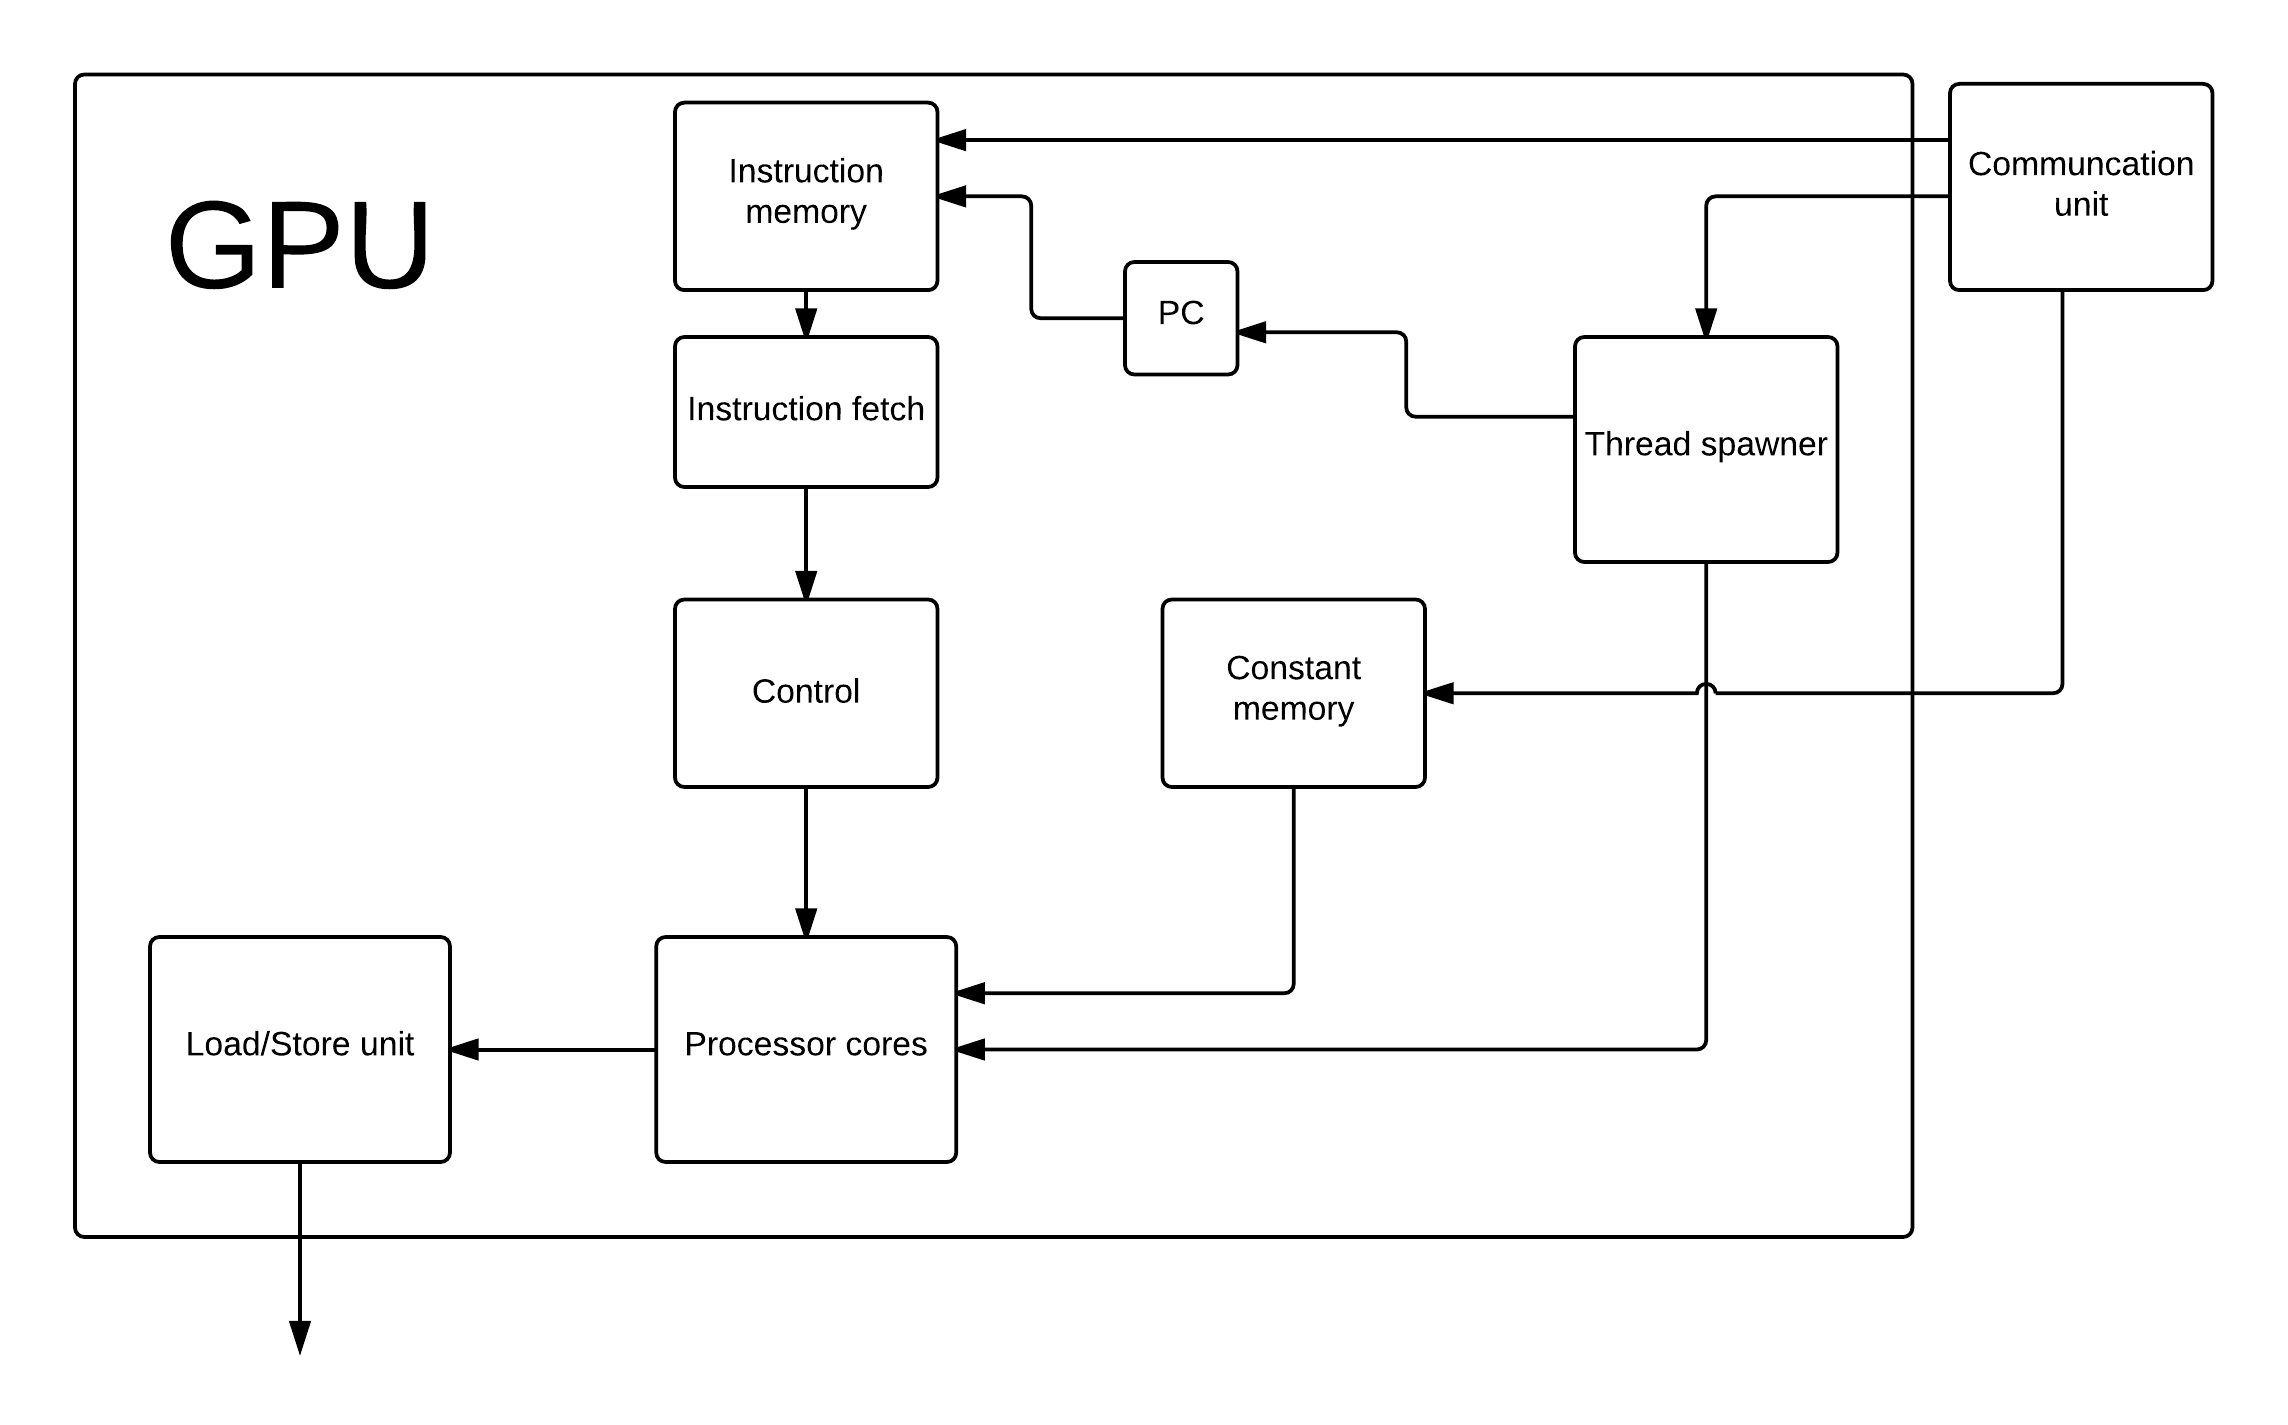
\includegraphics[width=\textwidth]{../gpu/diagrams/architecture_overview.png}
\caption{A high level overview of the GPU.}
\label{fig:architecture_overview}
\end{figure}

Figure \ref{fig:architecture_overview} presents a high level overview over the GPU.
The CPU issues commands to the communication unit in the GPU. Commands are launching a kernel, uploading kernels to the instruction memory, writing to the constant memory, and read/write to SRAM.
Instructions are fetched from the instruction memory and decoded by the control unit, which has the responsibility of setting the control signals for the instructions.
The control signals go to all 8 cores of the GPU, which can load constants from the constant memory, and use the load/store unit for accessing the data memory.


\section{Receiving a Kernel Call}
\begin{figure}[H]
\centering
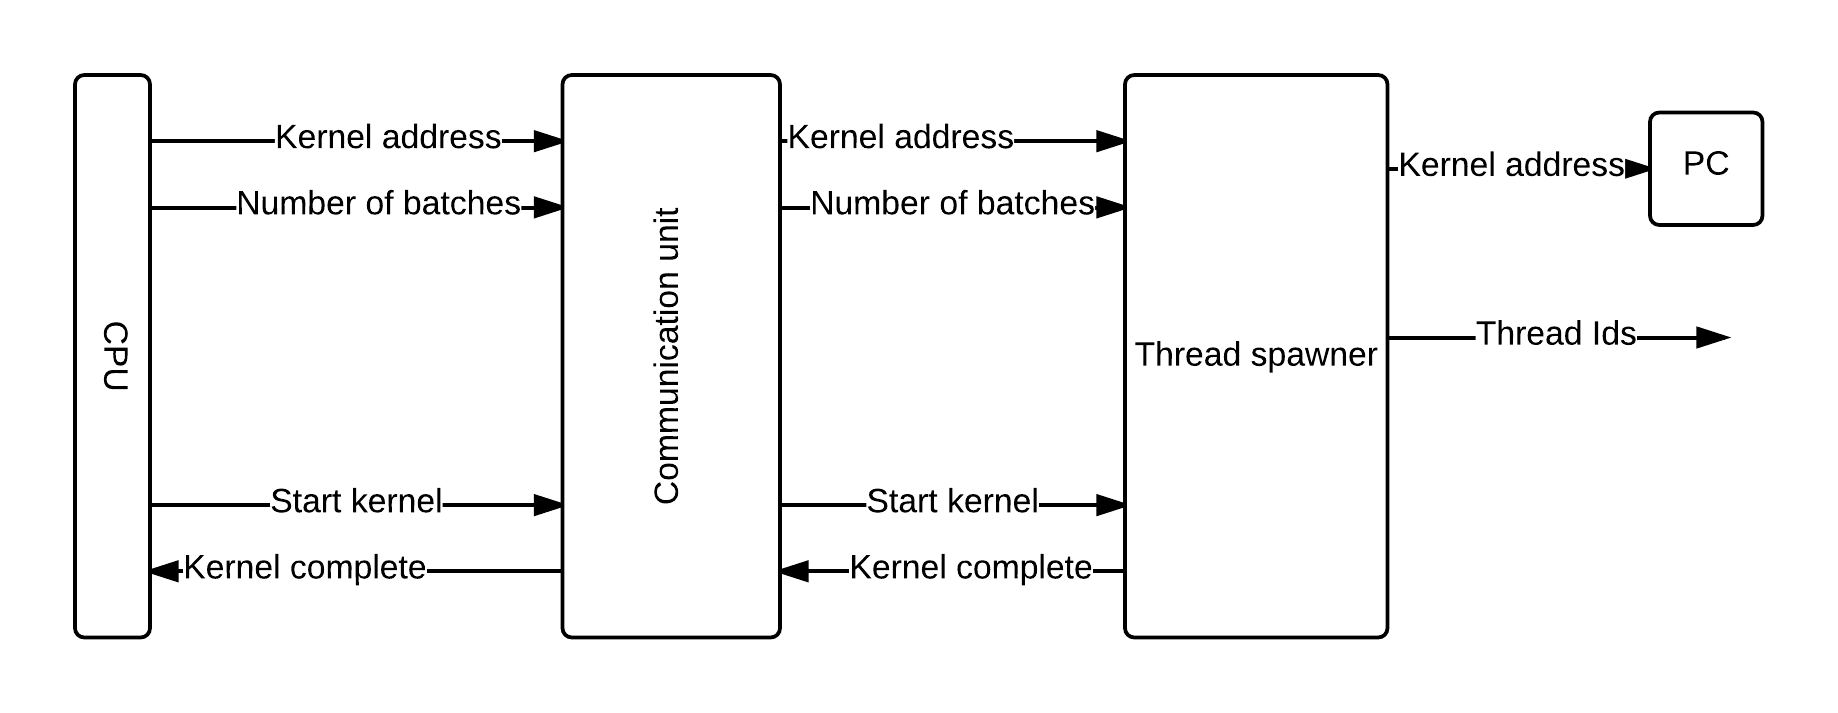
\includegraphics[width=\textwidth]{../gpu/diagrams/receiving_a_kernel_call.png}
\caption{Launching a kernel from the GPU's viewpoint.}
\label{fig:kernel_call}
\end{figure}

The communication unit is responsible for receiving kernel call requests from the CPU.
When a kernel call is received, the kernel launch signal is asserted.
A kernel call consists of the address of the kernel, and the number of threads to launch.

The kernel launch signals are forwarded to the thread spawner, which writes the kernel start address to the PC register, and starts distributing thread IDs to the processor cores. 
After holding the kernel launch signals high, the communication unit has completed its role in launching the kernel.
When the kernel completes executing, the thread spawner asserts the kernel done signal, and the communication unit forwards the signal to the CPU, indicating that the kernel call has completed.

\section{Running a Kernel}

\subsection{Warps}

As in NVIDIA's Fermi architecture, see chapter \ref{sec:fermi}, Demolicious organizes threads into \emph{warps}.
In Demolicious, a warp consists of 8 threads, one per core. 
For versions with fewer cores, the warp size changes accordingly.
Just as the warps in Fermi, every thread in these warps always execute the same instruction at the same time, with one thread in each core.
Note that while Fermi has multiple \emph{Streaming Multiprocessors} which can each execute warps concurrently, Demolicious can only execute a single warp at a time.
The Demolicious system is analogous to having a single Fermi \emph{Streaming Multiprocessor}.

An important difference between Demolicious and Fermi, is that Demolicious kernels have no jumps, so its threads never diverge.
This significantly reduces the complexity of scheduling these warps, and let's us get away with a single program counter.

\subsection{Static scheduling}

% Many mem requests per clock
As every thread in a warp always executes the same instruction, our system needs to handle 8 memory requests being issued during the same cycle.
The memory system for Demolicious consists of two SRAM chips, and can return two words every cycle.
%A memory request has a single cycle delay.
This bandwidth is not sufficient to satisfy the set of 8 memory requests produced by a warp without stalling.
Occasionally, these stalls can be hidden by the programmer if loads are issued ahead of their usage.
However, when the program does not have enough useful instructions to do while waiting for loads, the GPU must stall.
Stalling a throughput-oriented machine is obviously unfortunate.

\begin{figure}[htp]
\centering
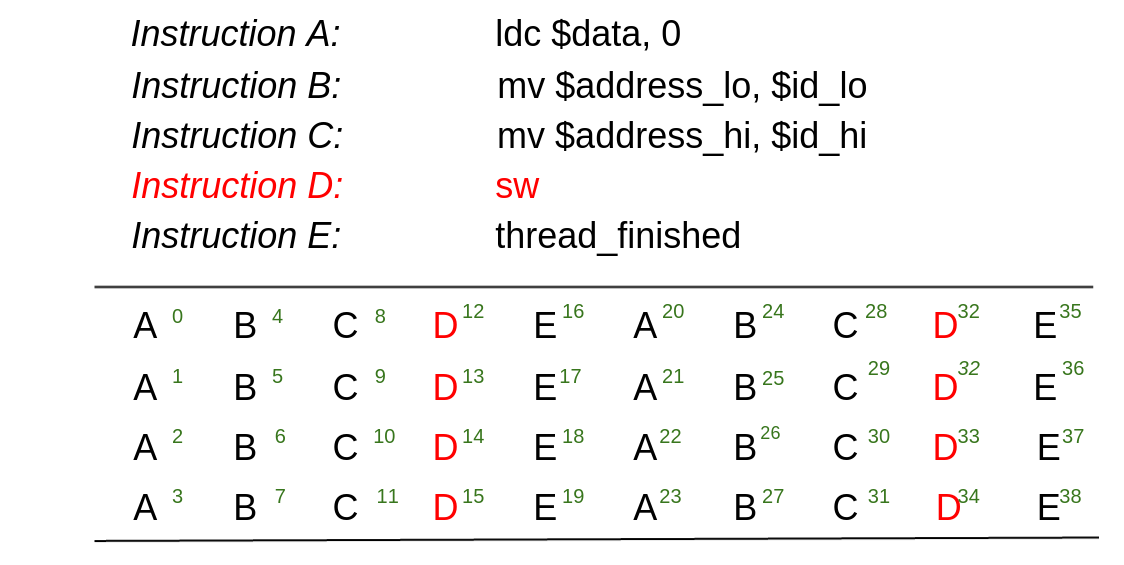
\includegraphics[scale=0.25]{../gpu/diagrams/uten_jaktstart_num.png}
\caption{Execution timing of warps without jagged scheduling}
\label{nojagged}
\end{figure}

\begin{figure}[htp]
\centering
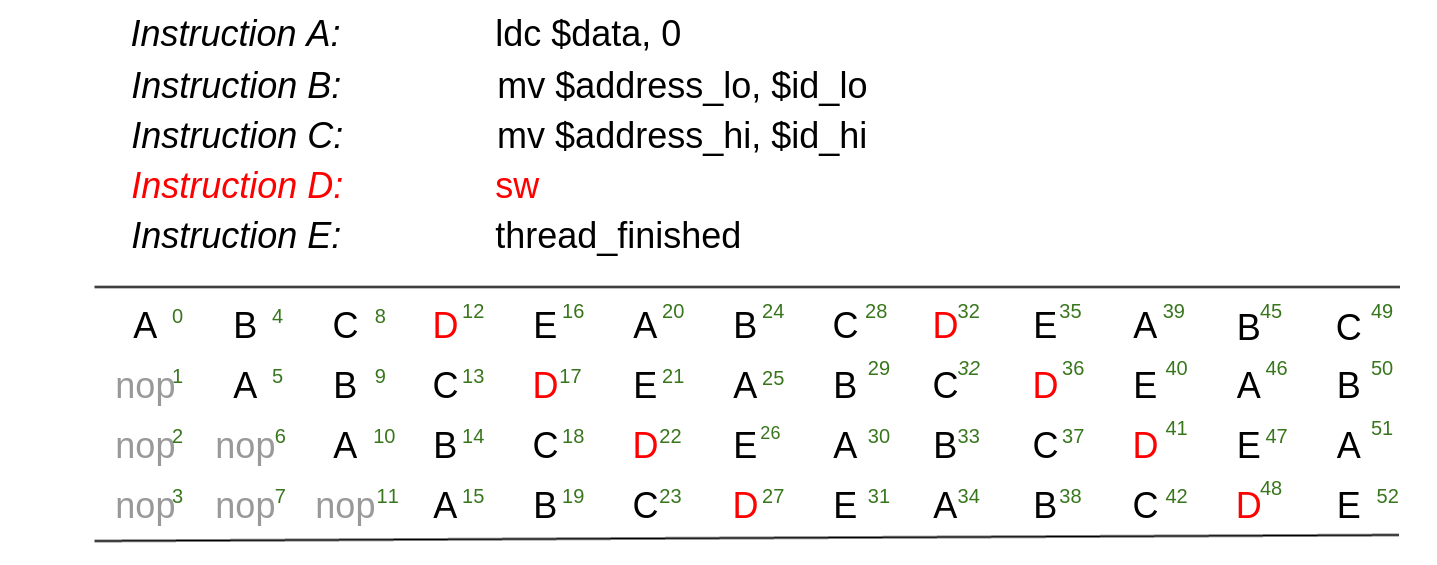
\includegraphics[scale=0.23]{../gpu/diagrams/jaktstart_num.png}
\caption{Execution timing of warps with jagged scheduling}
\label{jagged}
\end{figure}

But there are many warps waiting for execution at (almost) any time. 
If these warps could execute while other warps are waiting for memory, we can utilize the system better.
However, changing between warps that execute requires a context switch. 
That is, the old thread put on hold has to store all its register values somewhere so that they can be available when it starts executing again.
\todo{cite something?}
In software threading, a context switch is typically achieved by store all registers to memory and loading in the registers for the new thread that is scheduled.
This is an expensive operation, and would introduce more latency than we are trying to hide.
Demolicious, however, has a set of active warps that all have their own registers.
So a context switch can be carried out with virtually no overhead, at the expensive of some additional hardware to store all these extra registers.

To keep the architecture as simple, Demolicious employs a simple static scheduling algorithm. 
The active warps are simply rotated every instruction. In figure \ref{nojagged} we revisit our green-screen kernel, and see how the warps are scheduled. 
The numbers in the top right corner is the gpu cycle. 
During cycle 0, instruction A is executed on warp 0. 
The next cycle, instruction A is executed on warp 1. 
And when we get to cycle 4 warp 0 is scheduled again, this time executing instruction B.
This continues until we reach clock cycle 16-19 where warps 0 through 3 executes instruction E, the \emph{thread\_finished}, which does no computation, but allows the GPU to set up new warps.
On cycle 20, warp 4 is set up and ready to execute the first instruction.
This pattern continues untill all threads have run to completion. 

However, there is an issue with this simple scheduling algorithm. Let's see what happens when we get to instruction D, marked in red. In clock cycle 12\footnote{The cycle numbers are written in the upper right corner of each square} all threads in warp 0 executes a memory request, that is 8 memory requests. 
As our memory system handles two requests per clock, it is busy the next 4 cycles with this request, and when warp 0 gets to execute the next instruction, the memory operation is complete for all the threads.
Had this been a load instead of a store, it could be used on the next instruction, and we avoided a stall.
So far, so good.
However, when warp 1 executes the store instruction in cycle 13, the memory is already busy with the request from warp 0.
The memory requests from warp 1 cannot be started before cycle 16, and is not ready for its next instruction. 
It is even worse for warp 2 and 3. As all warps execute the same code, this can introduce up to 8 \emph{nop} instruction for every warp.

\begin{figure}[htp]
\centering
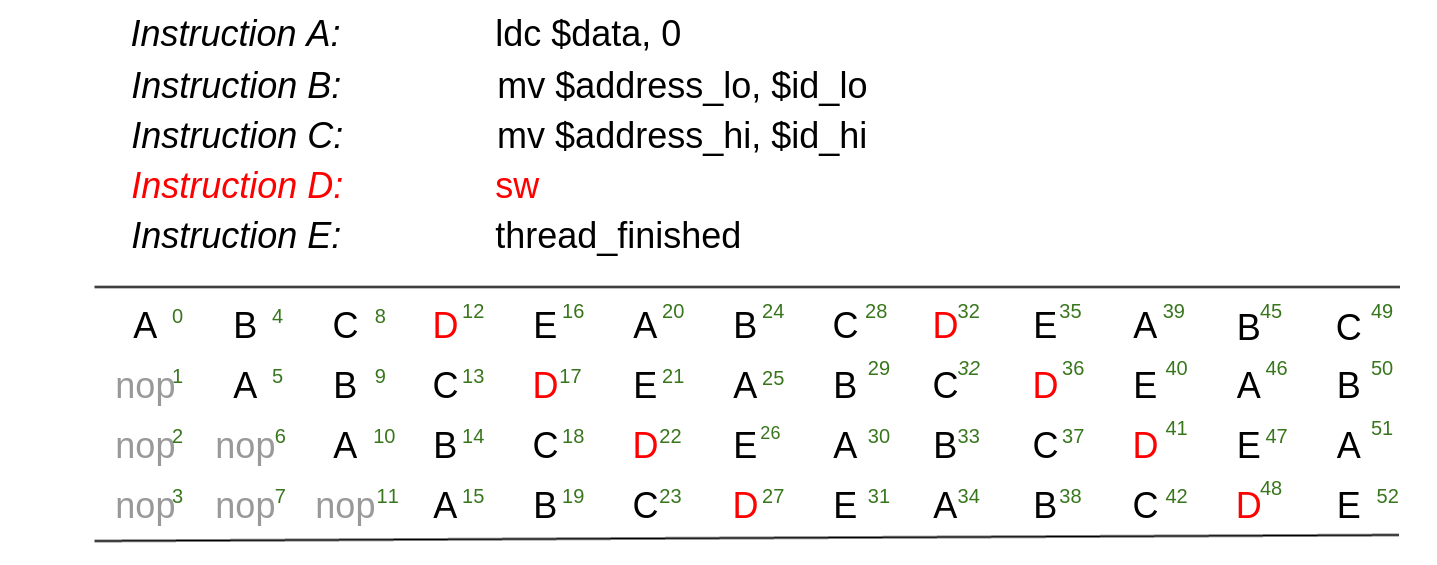
\includegraphics[scale=0.25]{../gpu/diagrams/jaktstart_num.png}
\caption{Execution timing of warps with jagged scheduling}
\label{jagged}
\end{figure}

Clearly, the introduction of this barrel processing technique did not solve our problems.
Fortunately, this was a simplified version of the scheduling in Demolicious. 
The actual scheduling is shown in figure \ref{jagged}. 
By introducing an offset in the instructions executed, henceforth called jagged execution\footnote{Or "jaktstart" as we like to call it in Norwegian}, we can avoid this issue.

With this scheduling, you can see that there are 4 executions without a memory operation between every memory operation.
This is true as long as memory operations have 4 non-memory operations between them in the kernel.
It is up to the programmer or assembler to ensure that this holds.


\subsection{Should this section be moved? What to call @}

Once the thread spawner has been initiated by the communication unit, the kernel runs to completion without intervention by the CPU. 
When a kernel run starts, the thread spawner assigns thread IDs to each warp in the barrel.
After the initial IDs have been assigned the GPU enters normal execution.
\begin{figure}[H]
    \centering
    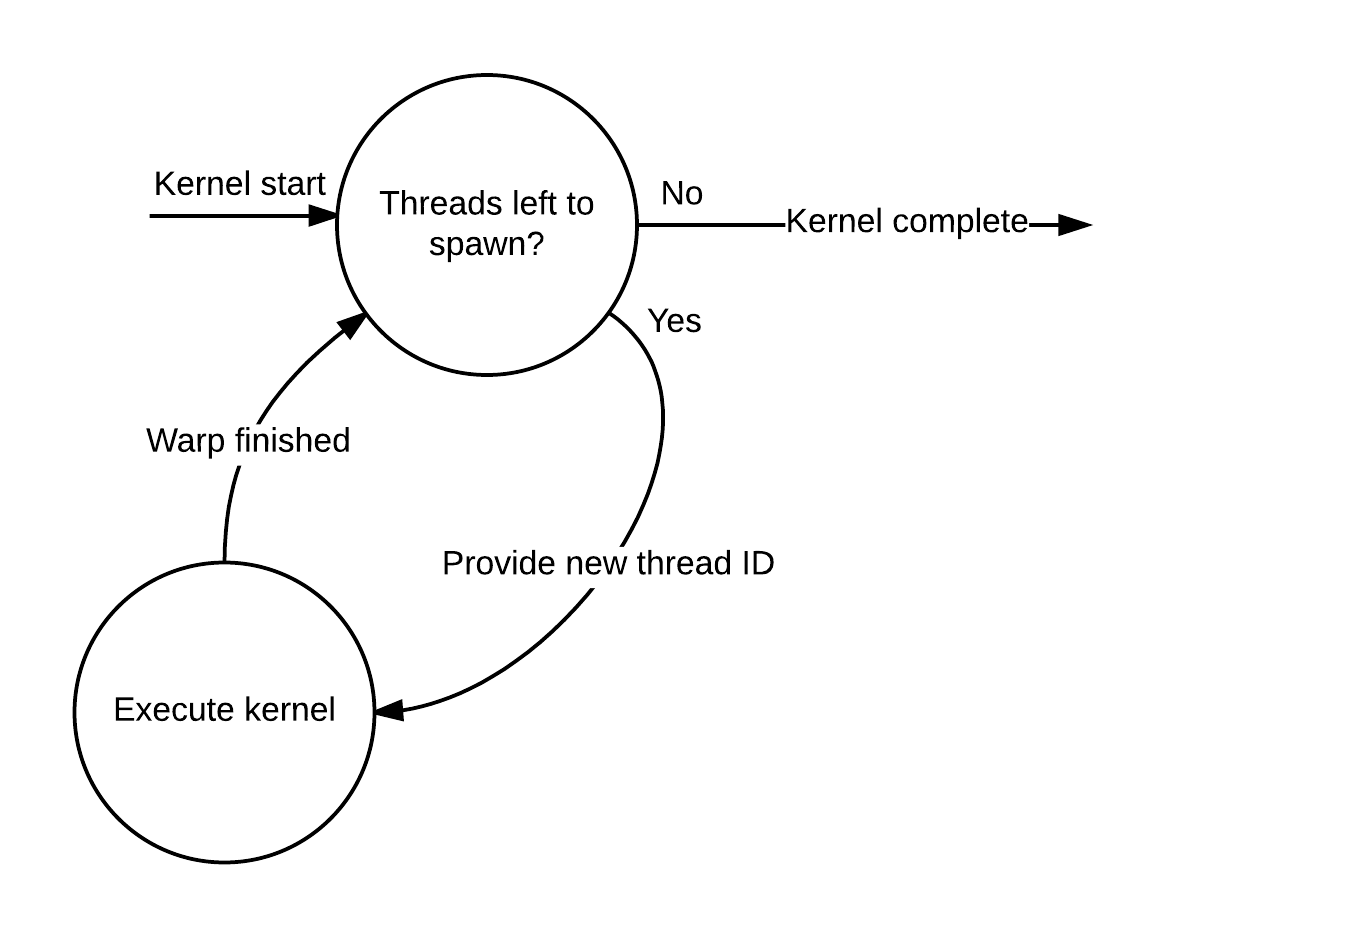
\includegraphics[width=0.9\textwidth]{../gpu/diagrams/kernel_run_state_machine.png}
    \caption{The GPU's internal state during kernel execution.}
    \label{fig:kernel_run_state_machine}
\end{figure}
A normal kernel execution can be represented by the state machine in figure \ref{fig:kernel_run_state_machine}.
During the kernel execution stage the threads in a warp execute the same instructions, until the control unit encounters a \emph{finished} instruction.
Upon receiving a \emph{finished} instruction the control unit asserts the \emph{finished} signal alerting the thread spawner that a new warp has to be spawned.
The thread spawner keeps track of the number of threads awaiting launch.
When the thread spawner receives a \emph{finished} instruction and no more warps are awaiting launch, the kernel complete signal is asserted, and the kernel run has completed.


\section{Module Details}

\subfile{../gpu/core.tex}

\subfile{../gpu/thread-spawner.tex}

\subfile{../gpu/regdir.tex}

\subfile{../gpu/sram.tex}

\subfile{../gpu/lsu.tex}

\subfile{../gpu/hdmi.tex}

\subsection{Summary}
The journey of our kernel is complete.
We have followed it all the way from the initial \emph{load\_kernel} call to the screen.
It has traveled through the massively parallel GPU which can handle a vast amount of threads,
by using hardware threads with a round-robin static scheduling technique called barrel processing.

\end{document}
